\PassOptionsToPackage{usenames,dvipsnames}{xcolor}
\documentclass[modern]{style_and_logos/lsstdescnote}
\usepackage{style_and_logos/lsstdesc_macros}
\pdfoutput=1 %for arXiv submission
\usepackage[T1]{fontenc}
\usepackage{ae,aecompl}
\usepackage[utf8]{inputenc}
\usepackage{newtxtext,newtxmath}
\usepackage[english]{babel}
\usepackage{amsmath,amstext,mathtools}
\usepackage[figure,figure*]{hypcap}
\usepackage[hang]{footmisc}
\setlength{\footnotemargin}{0.8em}
\usepackage{threeparttablex}
\usepackage{longtable}
\usepackage{inconsolata}
% change `finalizecache` to `frozencache` below for arxiv
\usepackage[finalizecache,cachedir=.]{minted}
\definecolor{DESCred}{rgb}{0.63,0.00,0.20}
\hypersetup{colorlinks=true,breaklinks=true,
  citecolor=DESCred,filecolor=DESCred,linkcolor=DESCred,urlcolor=DESCred}

% Commands for inserting attention-grabbing comments into the text.
\newcommand{\rachel}[1]{{\color{magenta}RM: #1}}
\newcommand{\mike}[1]{{\color{cyan}MJ: #1}}
\newcommand{\arun}[1]{{\color{blue}AK: #1}}

\shorttitle{PSFs of coadded images}

\begin{document}
\title{PSFs of coadded images}
\author[0000-0003-2271-1527]{Rachel Mandelbaum}
\affiliation{McWilliams Center for Cosmology, Department of Physics, Carnegie Mellon University, Pittsburgh, PA 15213, USA}
% Others to include if they agree:
\author[0000-0002-4179-5175]{Mike Jarvis}
\affiliation{Department of Physics \& Astronomy, University of Pennsylvania, 209 South 33rd Street, Philadelphia, PA 19104-6396, USA}
\author[0000-0003-1666-0962]{Robert H. Lupton}
\affiliation{Princeton University, Princeton, NJ, USA}
\author[0000-0003-2759-5764]{James Bosch}
\affiliation{Princeton University, Princeton, NJ, USA}
\author[0000-0001-8783-6529]{Arun Kannawadi}
\affiliation{Princeton University, Princeton, NJ, USA}

\date{\today}

\begin{abstract}
    We provide a detailed exploration of the connection between choice of coaddition schemes and the PSF of the coadd.  In particular, we investigate what properties of the coaddition algorithm lead to the coadd having a well-defined PSF.  The key elements of this discussion are as follows: 
    \begin{enumerate}
        \item We provide an illustration of how linear coaddition schemes can produce a coadd that lacks a well-defined PSF even for relatively simple scenarios and choices of weight functions.  
        \item We provide a more formal demonstration of the fact that a linear coadd only has a well-defined PSF in the case that either (a) each input image has the same PSF or (b) the coadd is produced with weights that are independent of the signal and the component PSFs.
        \item We discuss some reasons that two plausible nonlinear coaddition algorithms (median and clipped-mean) fail to produce a consistent PSF profile for stars.
        \item We demonstrate that all nonlinear coaddition procedures fail to produce a well-defined PSF for extended objects.
    \end{enumerate}
\end{abstract}
\maketitle

\section{Introduction}\label{sec:intro}

For many purposes, we currently use and will in future use coadded images to measure the properties of stars and galaxies observed in astronomical images.  The subject of this Note is the effective PSF of the coadded images, and in particular, {\em what is the impact of the algorithm used for coaddition on the effective PSF of the coadd?} Under what circumstances does the coadd have a well-defined PSF, and how is that PSF defined?  The answer to this question depends on (a) whether the coaddition scheme is linear or not (e.g., mean versus median), and (b) what weights are used for a linear coaddition scheme (e.g., including the object signal in an inverse variance weight). In particular, we will show that use of a nonlinear coaddition scheme and/or use of weights that include the signals of individual objects when carrying out a linear coaddition scheme results in a coadd that does not have a well-defined PSF.

For this purpose, we will ignore other relevant issues that occur in practice, such as the need to obtain an accurate astrometric solution in each exposure before producing the coadd, issues that can arise when carrying out the image registration and resampling through interpolation\footnote{This problem is particularly non-trivial for undersampled images.}, elimination of artifacts in individual exposures, magnitude-dependent detector effects that can modify the apparent PSF measured from stars, etc.  In other words, this writeup will assume that (a) the individual images are perfectly aligned with each other, (b) the PSF and its spatial variation are perfectly known in each individual exposure contributing to the coadd, (c) all detector non-idealities have been perfectly corrected, and (d) the coadd is produced at the native pixel scale. 
%Our formalism will, in addition, omit noise terms that are always present for real images. 
However, we will not assume that the individual exposures have the same PSF, as variation in PSF between exposures is what makes this problem of producing a coadd with a meaningful and well-understood PSF challenging. 
%Also, we will briefly touch on the issues that can arise when the coaddition algorithm is designed to eliminate artifacts by employing some nonlinear approach to coaddition, but will not delve into this issue extensively.

This topic has been discussed in the literature in many contexts, but unfortunately some of the key principles have not been explicitly demonstrated.  For example:
\begin{itemize}
\item \citet{2014ApJ...794..120A} provide some explanation but without mathematical justification in section 3.4: ``To keep track of the variance of data images, pixel by
pixel inverse variance images are a natural choice, but
they produce biases in the resulting mean. At low signal to noise the upward fluctuations in signal are given
more weight than downward fluctuations as a result of
the one-sided nature of the Poisson distribution. This
bias is deterministic and one could correct for it, but,
for example, for $u$-band data with its 120$e^{-}$ of sky noise,
pixels at $1\sigma$ above sky would be biased by 0.5\% and this
would be a fair fraction of our photometric error budget. Another problem is that per-pixel inverse variance
weighting systematically changes the shape of the PSF
as a function of the magnitude of the object.''  This is another way of saying there is no well-defined PSF for the resulting image.

\item \citet{2017ApJ...836..187Z} have a thorough discussion of the impact of coaddition choices on detection and measurements made on the coadd, but simply assert in their introduction that the variance used for weighting should be the `variance of all the background noise sources (e.g., background, readout noise)'.  This is an implicit rejection of weighting that includes information about the astronomical sources such as stars and galaxies, but without explanation. This work discusses a coaddition scheme that satisfies that criterion and that was proposed by Nick Kaiser in an unpublished tech note\footnote{\url{http://pan-starrs.ifa.hawaii.edu/project/people/kaiser/imageprocessing/im\%2B\%2B.pdf}}.

    \item \citet{2018ARA&A..56..393M} asserts without further explanation in section 2.4 that ``the coadd may not even have a well-defined PSF at each point (for example, inverse
variance weighting that depends on the total flux, or use of a median for the coadd). The
answer to this challenge is to generate the coadd in a principled way that results in a single
well-defined PSF at each point.''

\item \citet{2018PASJ...70S...5B} asserts without illustration in section 3.3.2 that ``For PSF model coaddition to be valid, the operation used to
combine all input pixels at each point on the coadd image must
be strictly linear – robust estimators such as the median or
sigma-clipped means cannot be used. Nonlinear estimators do
not just prevent PSF coaddition from working, however; they
prevent the coadd image from even having a well-defined effective PSF. Any estimator that rejects individual pixel outliers will tend to reject pixels in the cores of stars on the best-seeing exposures, and brighter stars will experience more rejection, giving
them a different profile than fainter stars. It should be emphasized that this occurs even in the absence of noise, and even
with extremely weak outlier rejection (e.g.\ clipping at $10\sigma$). All
robust estimators start from the ansatz that all input values are
drawn from the same underlying distribution, and convolution
with different PSFs means that they are not.''    

\item A tech note about coaddition algorithms\footnote{\url{https://dmtn-015.lsst.io/}} by Jim Bosch (for Rubin Observatory DM) states that when producing a coadd via a weighted summation over individual exposures, ``It is equally important that the weight function vary only on scales much larger than the size of the PSF; without this it the coadd has no well-defined effective PSF.'' \mike{I considered adding a [sic] here for the extra "it" in this sentence ("without this it the coadd...").  Can the original tech note be corrected?  Or should we perhaps silently fix the grammar here?}

\item \citet{2011ApJ...741...46R} note in section 2.2 that they derive a linear coadd estimator because this ``ensures that the final PSF ... is independent of image brightness, so the stars that were not used in the PSF determination are tracers of how well the image synthesis worked.''

\end{itemize}

In this Note we aim to provide some of the mathematical justification and physical intuition behind these statements, beginning with defining formalism in Section~\ref{sec:formalism}, then discussing linear and nonlinear coaddition schemes in Sections~\ref{sec:lin} and~\ref{sec:nonlin}, respectively.

\section{Formalism}\label{sec:formalism}

In this work we assume that multiple background-subtracted images $I_i(x,y)$ (with subscript $i$ indexing the individual images) are being combined to produce a coadded image $I_\text{coadd}(x,y)$.  Here the $(x,y)$ coordinates are not detector coordinates; they are meant to indicate some idealized sky coordinate system after correction for astrometric distortions on all scales. We also presume that each image has the same true underlying sky scene\footnote{This means that technically, our results only apply to static sources.  Following the results of this Note, it seems that the effective PSF on the coadd for time-varying sources will differ depending on the light curve (e.g., in the limit that a variable or transient source is very bright in just one exposure and faint in all the others, its PSF in the coadd will effectively be that of the exposure where it is very bright). If LSST is carried out with a `two snaps' approach then this is even relevant to how the two snaps are combined. Exploring these issues for time-varying sources is beyond the scope of this Note.} $T(x,y)$ (hence it has no index $i$) but a potentially different effective PSF\footnote{We use the phrase `effective PSF' to refer to the convolution of the PSF from the atmosphere and telescope optics with the pixel response function.  The effective PSF is then sampled at the centers of pixels.  We prefer this convention over the alternative, not including the pixel response and then explicitly integrating over the pixel response function, as it makes the bookkeeping cleaner for coadded or resampled images. Also note there is some ambiguity in the notation we are using for the $(x,y)$ argument of the effective PSF.  Here we mean that the effective PSF may vary as a function of position -- so when evaluating $P_i(x,y)$ at some specific $(x,y)$ position, we get a representation of the PSF that is also an image of some dimensionality.  (This is in contrast to $T(x,y)$, which when evaluated at a specific $x$ and $y$ is just a number.)} $P_i(x,y)$.  By definition, it is the case that
\begin{equation}
I_i(x,y) = T(x,y) \otimes P_i(x,y)    
\end{equation}
where $\otimes$ denotes convolution.

The question we wish to ask is under what circumstances does the coaddition process produce a coadded image such that there is a well defined function $P_\text{coadd}(x,y)$ that satisfies the condition
\begin{equation}\label{eq:coaddpsf}
    I_\text{coadd}(x,y) = T(x,y) \otimes P_\text{coadd}(x,y)
\end{equation}
or its Fourier-space equivalent 
\begin{equation}\label{eq:kcoaddpsf}
    \widetilde{I}_\text{coadd}(k_x,k_y) = \widetilde{T}(k_x,k_y) \widetilde{P}_\text{coadd}(k_x,k_y)?
\end{equation}

Each image is presumed to have a spatially-varying background level $B_i(x,y)$ that has been subtracted prior to PSF measurement and coaddition.  This background level can be used to define a spatially-varying weight function for coaddition.  Moreover, while not included explicitly as a separate term, each image is presumed to have noise.

\section{Linear coaddition schemes}\label{sec:lin}

In this section, we presume that the images are summed with weight functions $w_i(x,y)$, such that
\begin{equation}\label{eq:lincoadd}
    I_\text{coadd}(x,y) = \frac{\sum_i w_i(x,y) I_i(x,y)}{\sum_i w_i(x,y)}.
\end{equation}
The denominator ensures flux conservation in the coaddition process by enforcing that the effective weights $w_i/\sum_i w_i$ always sum to 1. Note that this is not the most general linear coadd estimator; a matrix product would be more general, and in the case of undersampled images, a matrix product is actually necessary to get a well-defined effective PSF \citep{2011ApJ...741...46R}.  However, for simplicity of notation we use Eq.~\eqref{eq:lincoadd} throughout this Note.

We begin with a direct illustration of the impact of weighting choices in a linear coaddition scheme, and then follow with a more formal demonstration of the circumstances under which the coadd has a well-defined PSF.

\subsection{Direct illustration}\label{subsec:direct}

\begin{figure}
\begin{center}
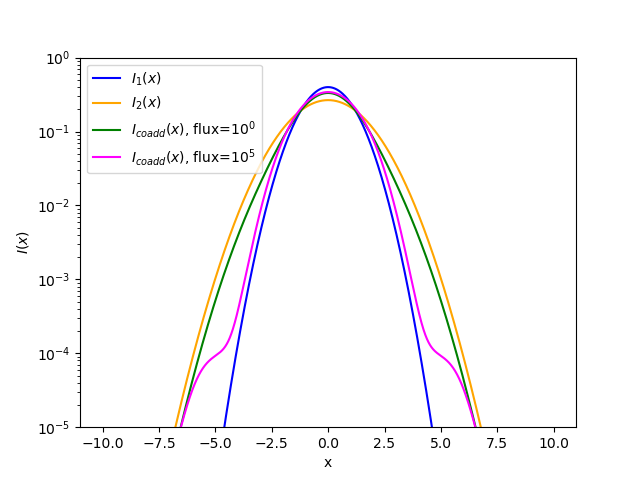
\includegraphics[width=5.5in]{figures/coadd_psf.png}
 \caption{Result of coadding two one-dimensional images of stars with different PSFs, depending on the total star flux $f_\text{star}$.  The figure shows the 1D images, all normalized to integrate to one for convenience of comparison, for the two star images $I_1(x)$ and $I_2(x)$ (Gaussians with $\sigma=1$ and $1.5$, respectively) and for the coadded images $I_\text{coadd}(x)$ produced assuming a constant background level of $10$ in each image, with inverse variance weighting from Eq.~\eqref{eq:optweight} including both background and signal.  As shown, the coadded images differ depending on whether the images are background-dominated (lower star flux, shown in green) or signal-dominated at the star center (higher star flux, shown in magenta).   } \label{fig:coadd_psf}
\end{center}
 \end{figure}
 
A natural choice for weighting is inverse variance weighting, to achieve an optimal signal-to-noise in the detection of objects in the coadd\footnote{Inverse variance weighting is {\em statistically} optimal unless one adopts more general linear coadd estimators involving a matrix product, as in the Kaiser approach.}.  We therefore define a fully spatially varying optimal weight for each image:
%while ensuring the weights sum to 1 at each point:
\begin{equation}\label{eq:optweight}
    w_{i,\text{opt}}(x,y) = \frac{1}{B_i(x,y)+I_i(x,y)}.
\end{equation}
Combining Eqs.~\eqref{eq:lincoadd} and~\eqref{eq:optweight}, the coadded image with this optimal weight is defined as
\begin{equation}\label{eq:optcoadd}
    I_\text{coadd,opt}(x,y) = \frac{\sum_i I_i(x,y)/\left[B_i(x,y)+I_i(x,y)\right]}{\sum_i 1/\left[B_i(x,y)+I_i(x,y)\right]}.
\end{equation}

To illustrate the impact of weight functions, we presume we are viewing an image of a single star.  In this case, we can assume that the sky scene consists of a delta function at the center of our image ($T(x,y)=f_\text{star}\delta(x=0,y=0)$) and therefore $I_i(x,y)=f_\text{star}P_i(x,y)$ where $f_\text{star}$ is the total star flux.  We further assume that the PSFs and backgrounds in the images will in general differ from each other, but are spatially constant, i.e., $B_i(x,y)=B_i$.  For simplicity, we consider PSFs that are described as Gaussians with $\sigma=1$ and $\sigma=1.5$ (arbitrary units), and just two images with a background level of $B_1=B_2=10$.  We then ask the question of what does the coadd look like for different values of $f_\text{star}$?  The result is shown in Figure~\ref{fig:coadd_psf}.

As shown, the resulting coadded image differs depending on whether the star flux is such that the images are background-dominated at all positions, or whether there are some positions near the center of the star that are signal-dominated.  This is a key result: in reality, there are objects of different fluxes throughout the images, and this figure suggests that once the images have different PSFs, the dependence of the weights on the flux means that objects will appear differently in the coadds depending on their brightness, even in the very simple case that we only have two images with the same constant background level and with a PSF that does not vary spatially within the images.  Once that is the case, there is no well-defined PSF for these images, as defined in Eq.~\eqref{eq:coaddpsf}.  Therefore, despite the statistical optimality of this weighting scheme, it is fundamentally flawed from the standpoint of systematics.

Ultimately the origin of these issues is that the weights that define the coadd in Eq.~\eqref{eq:optcoadd} depend on the input signal in the objects in the sky scene.  It seems possible that weights that depend only on quantities that are unrelated to the sky scene (example: background level and average seeing size) will not induce the same problems, which is the origin of the choices made in \citet{2014ApJ...794..120A} and \citet{2017ApJ...836..187Z}.  By extension, a coadd with weights that depend on object signals will come closer to having a well-defined PSF in the limit that all objects are background-dominated.

 \subsection{Formal demonstration}\label{subsec:formal}

 
 A more principled mathematical view of the issue comes from the relationship between these quantities in Fourier space.  Starting from Eq.~\eqref{eq:lincoadd}, we can use
 \begin{align*}
     I_\text{coadd}(x,y) &= \frac{\sum_i w_i(x,y) I_i(x,y)}{\sum_i w_i(x,y)} \\
     &= \frac{\sum_i w_i(x,y) \text{InvFT}[\widetilde{I}_i(k_x,k_y)]}{\sum_i w_i(x,y)}\\
     &= \frac{\sum_i w_i(x,y) \text{InvFT}[\widetilde{T}(k_x,k_y)\widetilde{P}_i(k_x,k_y)]}{\sum_i w_i(x,y)}.
 \end{align*}
And Eq.~\eqref{eq:coaddpsf} tells us that we want to know when is there some function $\widetilde{P}_\text{coadd}(k_x,k_y)$ such that
\begin{equation*}
    I_\text{coadd}(x,y) = \text{InvFT}[\widetilde{T}(k_x,k_y)\widetilde{P}_\text{coadd}(k_x,k_y)]?
\end{equation*}
We could imagine trying to find $\widetilde{P}_\text{coadd}$ via division,
\begin{equation}\label{eq:fourier_solve}
    \widetilde{P}_\text{coadd}(k_x,k_y) = \frac{\widetilde{I}_\text{coadd}(k_x,k_y)}{\widetilde{T}(k_x,k_y)}.
\end{equation}
However, for there to be a valid PSF, it needs to be the case that the true scene divides out of this ratio.  It seems that for a completely general set of weights to result in a well-defined PSF for the coadd, $\widetilde{I}_\text{coadd}(k_x,k_y)$ must include the scene in the form of a straightforward product.  Or, equivalently, it must be possible to write $I_\text{coadd}(x,y)$ as the convolution of the true scene and some other function.   For a linear coaddition scheme, this will only occur under the following conditions:
\begin{itemize}
    \item \textbf{Same PSF in each image:} If all the component exposures have the same PSF (possible, e.g., for space-based observations, where there is no atmosphere, if there is very little dithering between the exposures), then we have $P_i(x,y)=P(x,y)$.  In this case, Eq.~\eqref{eq:lincoadd} reduces to
    \begin{align*}
         I_\text{coadd}(x,y) &= \frac{\sum_i w_i(x,y) T(x,y)\otimes P(x,y)}{\sum_i w_i(x,y)} \\
         &= T(x,y)\otimes P(x,y).
    \end{align*}
    Since each image has the same PSF, they are all the same (modulo noise).  Hence the sum over the spatially varying weight function in each image cancels out of the numerator and denominator, and has no impact on the PSF of the resulting coadd.  The coadded image has a well-defined PSF: it is the same as the PSF in each input image.
    
    \item \textbf{Spatially constant weight functions:}  If the weight for each exposure is not a function of position on the exposure, then  $w_i(x,y)=w_i$.  In this case, we can rewrite Eq.~\eqref{eq:lincoadd} as
    \begin{align}
        I_\text{coadd}(x,y) &= \frac{\sum_i w_i I_i(x,y)}{\sum_i w_i} \nonumber\\
        &= \frac{\sum_i w_i \left[T(x,y) \otimes P_i(x,y)\right]}{\sum_i w_i} \nonumber \\
        &= T(x,y) \otimes \frac{\sum_i w_i P_i(x,y)}{\sum_i w_i},\label{eq:constweight}
    \end{align}
    where the last step relies on the linearity of convolution.  
    Eq.~\eqref{eq:constweight} shows that in this case, the scene is included in $I_\text{coadd}(x,y)$ as a direct convolution, which means the coadd has a well-defined PSF, 
    \begin{equation}\label{eq:constweightpsf}
        P_\text{coadd}(x,y) = \frac{\sum_i w_i P_i(x,y)}{\sum_i w_i}.
    \end{equation}

    \item \textbf{Weights that are independent of the true scene or the PSF:}  If the weights are based solely on imaging characteristics (e.g., the background level, electronic read noise, etc.), and not anything correlated with the true scene or the PSF, then the weights $w_i(x,y)$ are uncorrelated with both $T(x,y)$ and $P_i(x,y)$.
    In this case, we have $\langle (w_i(x,y)-\bar w_i) T(x,y) \rangle = 0$ and $\langle (w_i(x,y) - \bar w_i) P_i(x,y) \rangle = 0$, where $\tilde{w_i} = \langle w_i(x,y)\rangle$, the spatial average of the weights.  
    
    Define $P_\text{coadd}$ to be the weighted average PSF:
    \begin{equation}\label{eq:varweightpsf}
        P_\text{coadd}(x,y) = \frac{\sum_i w_i(x,y) P_i(x,y)}{\sum_i w_i(x,y)}.
    \end{equation}
    It won't be the case now that we can satisfy Eq.~\eqref{eq:coaddpsf} specifically at every location, since $\widetilde{T}$ will not cancel out in Eq.~\eqref{eq:fourier_solve}, but we can satisfy it in an expectation-value sense:
    \begin{align*}
      &\left\langle I_\text{coadd}(x,y) - T(x,y) \otimes P_\text{coadd}(x,y) \right\rangle \\
      &\qquad= \Bigg\langle \frac{
                  \sum_i w_i(x,y) \int dx^\prime dy^\prime T(x^\prime,y^\prime) P_i(x-x^\prime,y-y^\prime)  }{\sum_i w_i(x,y)} \qquad \\
      &\qquad \qquad - \frac{\int dx^\prime dy^\prime T(x^\prime,y^\prime) \sum_i w_i(x-x^\prime,y-y^\prime) P_i(x-x^\prime,y-y^\prime)}{\sum_i w_i(x,y)} \Bigg\rangle \\
      &\qquad= \left\langle\frac{
                  \sum_i \int dx^\prime dy^\prime T(x^\prime,y^\prime) P_i(x-x^\prime,y-y^\prime) (w_i(x,y) - w_i(x-x^\prime,y-y^\prime)}{\sum_i w_i(x,y)} \right\rangle \\
      &\qquad= \frac{
                  \sum_i \int dx^\prime dy^\prime T(x^\prime,y^\prime) P_i(x-x^\prime,y-y^\prime) \left\langle w_i(x,y) - w_i(x-x^\prime,y-y^\prime)\right\rangle}{\sum_i w_i(x,y)} \\
      &\qquad= 0
    \end{align*}
    where the second step relies on $w_i$ being uncorrelated with $T$ and $P_i$.
    
    Thus, in this case, we have the slightly modified condition:
    \begin{equation}\label{eq:expcoaddpsf}
        \left\langle I_\text{coadd}(x,y) \right\rangle = \left\langle T(x,y) \otimes P_\text{coadd}(x,y) \right\rangle
    \end{equation}
    Each location on the image will not specifically follow Eq.~\eqref{eq:coaddpsf}, but using this equation as a model of the observed coadd image will be unbiased when applied to a large ensemble of sources.  For most purposes, this is a sufficient definition for there being a well-defined PSF.

\end{itemize}
These are the only options that guarantee that the linear coadd defined in Eq.~\eqref{eq:lincoadd} can be rewritten as the convolution of the true sky scene with some other function. In any other case, it is not possible to guarantee that the coadded image will have a well-defined PSF.
%\rachel{Unless I am missing something?} \mike{I couldn't think of any other cases that worked out either, but I don't immediately see a real proof of this claim.}

\begin{figure}
\begin{center}
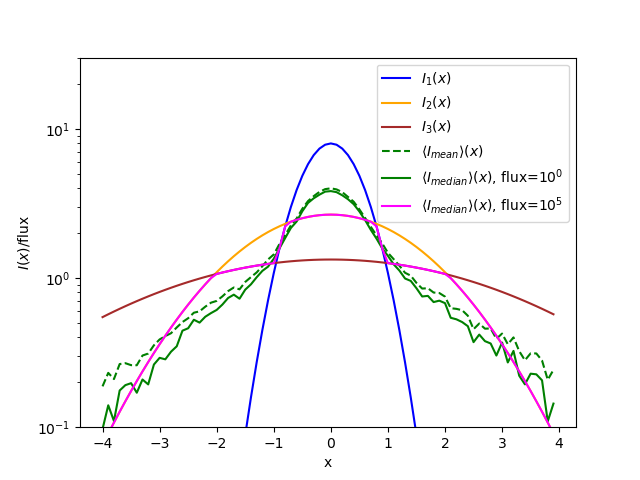
\includegraphics[width=5in]{figures/noisy_median_coadd_psf.png}
 \caption{Result of applying a median coaddition procedure to three one-dimensional images of stars with different PSFs. 
 First, we show the images for three one-dimensional Gaussian images with different PSFs (denoted $I_i(x)$ in the legend) -- with the flux divided out to avoid stars of different fluxes requiring very different axes.  The other curves show the average coadd profile from many noisy realizations, including a sky background of 100.  The dashed curve shows an unweighted mean coadd profile (for any star flux), which has a well-defined PSF.  The solid green curve shows the result for a median coadd for a low-flux (background-dominated) star, which as shown looks very similar to the mean coadd.  Finally, the pink curve shows the result for the median coadd for a high-flux (signal-dominated) star.  
 The fact that the pink and green curves differ demonstrates that there is no well-defined PSF for a median coadd.
 }
 \label{fig:median_coadd_psf}
\end{center}
 \end{figure}

In reality, it will never be the case that each image has precisely the same PSF; therefore, selecting spatially constant weight functions, or at least weight functions that are independent of $T$ and $P_i$, provides a viable route to ensuring the coadd has a well-defined PSF.  
In practice, the last option seems to be the most common, since the various references in Section~\ref{sec:intro} of this Note accept the idea of weighting by the spatially-varying background, with the DM tech note providing an approximate criterion: the weight function should ``vary only on scales much larger than the size of the PSF.''  This criterion helps guarantee that the weights will be uncorrelated with the sources, at least for the small objects that are typically used for dark energy science.
%\rachel{We could explore this a little more with our formalism, with a weight function $w_i(x,y)$ to which we have applied a low-pass filter, and show what that does -- is this useful?}

\section{Nonlinear coaddition schemes}\label{sec:nonlin}

There are several possible nonlinear coaddition schemes that one might consider adopting in reality.  While the discussion in Sec.~\ref{subsec:formal} makes it challenging to envision a nonlinear approach that would result in a well-defined PSF for the coadd, we discuss the specific issues with two potential nonlinear approaches below before explaining mathematically why it is impossible for a nonlinear coadd scheme to have a well-defined PSF.

\subsection{Median coadds}

In order to avoid contamination by image artifacts, one possible `robust statistic' is a median rather than a mean.  In Figure~\ref{fig:median_coadd_psf} we illustrate the hazards of a median approach.
We show the images for three one-dimensional Gaussian images with different PSFs, along with the profile generated by a median coadd.  We generated $5\times 10^5$ noisy realizations of the images with a sky background of 100,  used them to make coadds, and then took the average of that coadd across all of those realizations to beat down the noise.  This was done for both low- and high-flux stars (flux = $1$ and $10^5$ respectively).
As shown, the high-flux case results in a star image with discontinuous slope, as expected from the medians of the three noise-free star images.  In contrast, in the low-flux case, the star image resembles an unweighted mean coadd. 
This illustrates that the PSF depends on the object magnitude, meaning that the coadd does not have a single well-defined PSF.

\subsection{Clipped-mean coadd}

Another obvious `robust statistic' to try is a clipped mean, i.e., defining some $\sigma$ value (through an IQR or direct calculation), and omitting pixels from an image if they deviate from the mean by more than $N\sigma$, possibly working iteratively until convergence is achieved.

However, as noted in Sec.~\ref{sec:intro}, \citet{2018PASJ...70S...5B} has pointed out the issues with clipped means.  Functionally, they are the solution to a different problem, one where all of the data are drawn from the same underlying distribution.  In the case of coaddition, different images have different PSFs, so the observed sky is drawn from a different distribution.  For example, images with a smaller PSF will preferentially have higher pixel values at the centers of bright stars and galaxies, which will preferentially fail such an $N\sigma$ criterion orders of magnitude more frequently than one would expect for a Gaussian distribution in cases where the data are drawn from the same underlying distribution.  Omitting data preferentially as a function of PSF size, especially doing so differently for different parts of an object (i.e. core vs. wings), will naturally result in a coadd with no well-defined PSF. This is true even for relatively large values such as $N=10$.  

\subsection{Extended Sources}

The above arguments about median and clipped-mean coadds seem to imply that they are only a
problem at moderately low signal-to-noise.  At high signal-to-noise, the profiles of stars are nearly
independent of the flux of the star for both median and clipped-mean coadds.  
However, when considering extended sources (i.e. galaxies),
there is an additional problem with these, or indeed any, nonlinear coaddition schemes,
even when limiting to high signal-to-noise sources.

We typically determine the PSF profile by looking at the images of stars, since these represent
the response of the imaging process to a delta function.  This essentially acts like a
Green's function of the imaging ``operator''.
\begin{equation}
    P_i(x,y) = \mathbf{F}_i \delta(x,y)
\end{equation}
for some potentially complicated imaging process $\mathbf{F}_i$.

We can then model the same process acting on an extended object
\begin{equation}
    I_i(x,y) = \mathbf{F}_i T(x,y)
\end{equation}
as a convolution
\begin{align}
    I_i(x,y) &= \mathbf{F}_i \int T(x^\prime,y^\prime) \delta(x-x^\prime,y-y^\prime) \nonumber\\
    &= \int T(x^\prime,y^\prime) \mathbf{F}_i \delta(x-x^\prime,y-y^\prime) \nonumber\\
    &= \int T(x^\prime,y^\prime) P_i(x-x^\prime,y-y^\prime) \nonumber\\
    &= T(x,y) \otimes P_i(x,y),
\end{align}
which is valid so long as $\mathbf{F}_i$ is a linear operator.

When we coadd multiple images $I_i(x,y)$ into $I_\mathrm{coadd}(x,y)$, this coadding process
essentially becomes part of the imaging operator $\mathbf{F}_\mathrm{coadd}$.
\begin{align}
    I_\mathrm{coadd}(x,y) &= \mathrm{Coadd} \left( \{ I_i(x,y) \} \right) \nonumber\\
    &= \mathrm{Coadd} \left( \{ \mathbf{F}_i(x,y) T(x,y) \} \right) \nonumber\\
    &\equiv \mathbf{F}_\mathrm{coadd} T(x,y).
\end{align}
When applied to stars, after normalizing the images by their fluxes,
we can call the resulting profile $P_\mathrm{coadd}$, but as we will see, this is
not really a PSF when $\mathbf{F}_\mathrm{coadd}$ is nonlinear.
\begin{align}
    P_\mathrm{coadd}(x,y) &= \mathrm{Coadd} \left( \{ P_i(x,y) \} \right) \nonumber\\
    &= \mathrm{Coadd} \left( \{ \mathbf{F}_i(x,y) \delta(x,y) \} \right) \nonumber\\
    &= \mathbf{F}_\mathrm{coadd} \delta(x,y).
\end{align}
If the coadd process is not a linear combination of the inputs, 
then $\mathbf{F}_\mathrm{coadd}$ is not a linear operator, and it is no longer valid to
write $I_\mathrm{coadd}$ as a convolution of $P_\mathrm{coadd}$:
\begin{align}
    I_\mathrm{coadd}(x,y) &= \mathbf{F}_\mathrm{coadd} \int T(x^\prime,y^\prime) \delta(x-x^\prime,y-y^\prime) \nonumber\\
    &\ne \int T(x^\prime,y^\prime) \left( \mathbf{F}_\mathrm{coadd} \delta(x-x^\prime,y-y^\prime) \right) \nonumber\\
    I_\mathrm{coadd}(x,y) &\ne T(x,y) \otimes P_\mathrm{coadd}(x,y).
\end{align}


\begin{figure}
\begin{center}
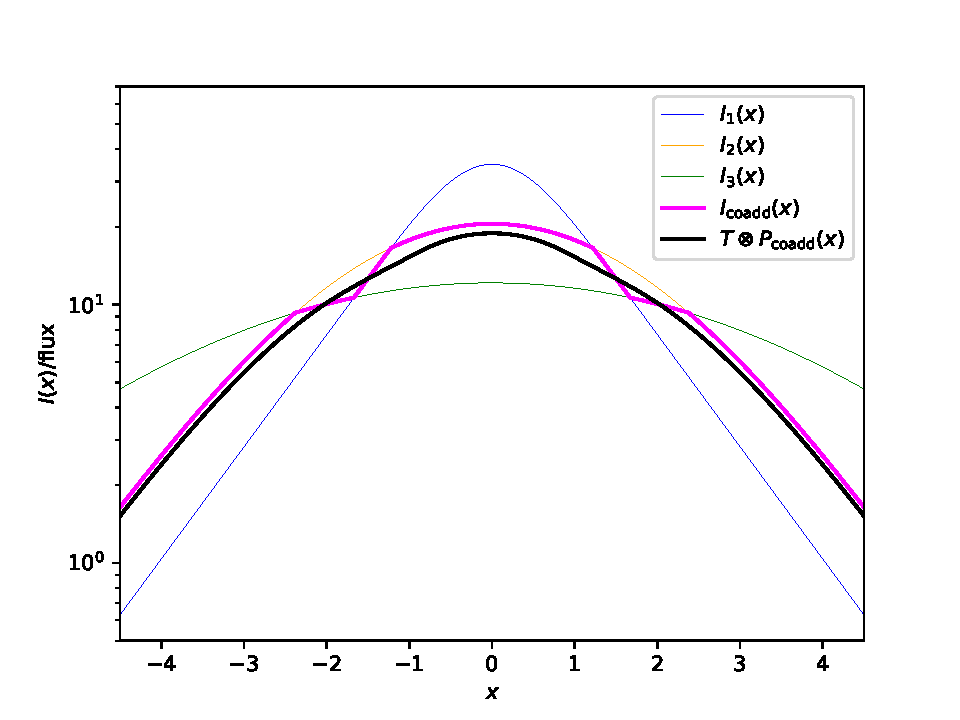
\includegraphics[width=5in]{figures/extended.pdf}
 \caption{The effect of using a median coadd on an extended object. 
 The thin blue, orange, and green curves show a single exponential galaxy profile convolved by the 
 same three PSF profiles as shown in Figure~\ref{fig:median_coadd_psf}. The magenta curve is the result
 of using a median coadd procedure on these images.  The black curve is the convolution of the true
 galaxy profile with the inferred PSF from the mean stellar profile at high signal-to-noise (i.e. the magenta profile in Figure~\ref{fig:median_coadd_psf}).  The fact that the
 black and magenta curves differ shows that even at high signal-to-noise, nonlinear coaddition algorithms
 (like median) do not result in a well-defined PSF.} \label{fig:extended}
\end{center}
 \end{figure}

Thus, when the coadd process is not linear,
the coadd image of an extended source is {\bf not} the convolution of the true scene by what
we would want to call the PSF.
Essentially, the entire concept of what we mean by a ``point-spread function'' (i.e. the response
of the imaging operator to a delta function, or ``point'') is invalid for a nonlinear imaging operator.  
Since the coaddition process is properly included as part of this operator, if that
step is nonlinear, then there is no well-defined PSF. 
Figure~\ref{fig:extended} demonstrates this fact for an exponential galaxy profile using a median
coaddition process (using the same three PSFs as shown in Figure~\ref{fig:median_coadd_psf}).

\section{Conclusion}

In this note, we showed a number of choices in coaddition algorithm that could result
in the coadd image not having a well-defined PSF, by which we mean that there is no
PSF function one can define for each location in the coadd such that the observed image is a convolution
of the true scene with this PSF.\arun{In general, for a PSF to be well-defined, the coaddition procedure must preserve linearity and translational-invariance. Non-linear coaddition algorithms violate the linearity condition, and per-pixel weighting violates the latter.}

We note that not having a well-defined PSF is not necessarily a problem always.  There are many use cases for coadd images
where one does not care whether the PSF is well-defined.  E.g. making color images
for showing observations of a planetary nebula, or possibly detection coadds where one may just want to maximize total signal-to-noise.
%\mike{??  I feel like at least some detection coadds might want a well-defined PSF, but maybe sometimes you don't really care?} \rachel{I think you are right, but since it says `possibly' and `may', I think it allows for the possibility that one may indeed want a well-defined PSF for a detection coadd in some cases.}
But for almost any use case where one will
be making some measurement (e.g., flux or shape) based on the pixel values in the coadd,
it is essential to have a well-defined PSF.  In these cases, the tradeoff between systematic and statistical uncertainties may point towards choices that are less statistically optimal (e.g., no use of inverse variance weights that include the object flux) but that reduce systematics.  Note, moreover, that this has implications for steps that may often be considered part of a process that precedes coaddition, such as cosmic ray rejection (see, for example, the discussion in section 3.3 of \citealt{2018PASJ...70S...5B}).

We found that the following choices in the coadd algorithm lead to the coadd failing to
have a well-defined PSF:
\begin{itemize}
    \item All nonlinear coadd algorithms fail to have a well-defined PSF.  The coadd procedure is essentially part of the total imaging process, so if that is not linear in the inputs, then the final profiles of extended objects are not the convolution of the true scene with the profile of a delta function ("point"), thus invalidating the whole idea of a "point-spread function".
    \item Even for point sources, nonlinear coadd algorithms essentially change their expectation value as a function of signal-to-noise, so the expected profile is not independent of flux.  Thus, they do not have a well-defined PSF even when only applied to stars.
    \item Linear coadd algorithms fail to have a well-defined PSF if their weights are a function of the signal.  This means if one is using inverse variance weighting, one should not include the Poisson noise of the signal as part of that variance.
    \item Similarly, the weights should not be a function of the PSF profiles of the input exposures, as this can also lead to biases in the measured properties of the coadd images.
    \item Technically, any weight function that is not spatially constant on each source image leads to the final image not having a formally well-defined PSF in the sense of following Eq.~\eqref{eq:coaddpsf}.  In practice this is usually not a problem in an expectation-value sense, so long as the spatial variability of the weights is uncorrelated with the input signal and the component PSF functions.  In this case, the coadd image follows Eq.~\eqref{eq:expcoaddpsf}. The non-uniform weights can add some additional scatter in the observed $I_\mathrm{coadd}(x,y)$, but not a bias.  For most use cases, this is acceptable.
\end{itemize}

Given these constraints, we are left only with linear coadd schemes using weights that are independent of the signal and the component PSFs.  If one needs the coadd PSF to be specifically correct at every location in the image, rather than merely unbiased, then one should use spatially invariant weights; however, this is typically not necessary. Note that we did not go into detail about matrix-based coadds, but these also qualify as linear, so these can be perfectly valid, so long as the matrix of weights follows the same restrictions of being independent of the signal and PSFs.

\section*{Acknowledgments}

We thank Chris Stubbs, Xiangchong Li, and Morgan Schmitz for useful feedback on a draft of this Note.

\bibliographystyle{style_and_logos/apj}
\bibliography{main}  

\end{document}
